%%%%%%%%%%%%%%%%%%%%%%%%%%%%%%%%%%%%%%%%%
% Short Sectioned Assignment
% LaTeX Template
% Version 1.0 (5/5/12)
%
% This template has been downloaded from:
% http://www.LaTeXTemplates.com
%
% Original author:
% Frits Wenneker (http://www.howtotex.com)
%
% License:
% CC BY-NC-SA 3.0 (http://creativecommons.org/licenses/by-nc-sa/3.0/)
%
%%%%%%%%%%%%%%%%%%%%%%%%%%%%%%%%%%%%%%%%%

%----------------------------------------------------------------------------------------
%	PACKAGES AND OTHER DOCUMENT CONFIGURATIONS
%----------------------------------------------------------------------------------------

\documentclass[paper=a4, fontsize=11pt]{scrartcl} % A4 paper and 11pt font size

\usepackage[T1]{fontenc} % Use 8-bit encoding that has 256 glyphs
\usepackage{fourier} % Use the Adobe Utopia font for the document - comment this line to return to the LaTeX default
\usepackage[english]{babel} % English language/hyphenation
\usepackage{amsmath,amsfonts,amsthm} % Math packages

\usepackage{lipsum} % Used for inserting dummy 'Lorem ipsum' text into the template

\usepackage{sectsty} % Allows customizing section commands
\allsectionsfont{\centering \normalfont\scshape} % Make all sections centered, the default font and small caps

\usepackage{fancyhdr} % Custom headers and footers
\usepackage{bm}
\usepackage{upgreek}
\usepackage{tikz}
\usetikzlibrary{shapes, arrows}
\pagestyle{fancyplain} % Makes all pages in the document conform to the custom headers and footers
\fancyhead{} % No page header - if you want one, create it in the same way as the footers below
\fancyfoot[L]{} % Empty left footer
\fancyfoot[C]{} % Empty center footer
\fancyfoot[R]{\thepage} % Page numbering for right footer
\renewcommand{\headrulewidth}{0pt} % Remove header underlines
\renewcommand{\footrulewidth}{0pt} % Remove footer underlines
\setlength{\headheight}{13.6pt} % Customize the height of the header

\setlength\parindent{0pt} % Removes all indentation from paragraphs - comment this line for an assignment with lots of text

%----------------------------------------------------------------------------------------
%	TITLE SECTION
%----------------------------------------------------------------------------------------

\newcommand{\horrule}[1]{\rule{\linewidth}{#1}} % Create horizontal rule command with 1 argument of height

\title{
\normalfont \normalsize
\textsc{MAGICC Lab - Brigham Young University} \\ [25pt] % Your university, school and/or department name(s)
\horrule{0.5pt} \\[0.4cm] % Thin top horizontal rule
\huge Mixer \\ % The assignment title
\horrule{2pt} \\[0.5cm] % Thick bottom horizontal rule
}

\author{James Jackson} % Your name

\date{\normalsize\today} % Today's date or a custom date

\begin{document}

\maketitle % Print the title

%----------------------------------------------------------------------------------------
%	PROBLEM 1
%----------------------------------------------------------------------------------------

\section{Introduction}

The mixer is a mechanism by which abstract roll rate, pitch rate, yaw rate and throttle commands are mapped to the actuators of the MAV.  In it's simplest form, the mixer is simply a matrix multiplication which maps these inputs onto motor outputs.

In addition to the mixer, there is some saturation functionality baked into ROSflight.  This functionality is insipired by that implemented in cleanflight, and serves to ensure that the MAV is always capable of responding to inputs, even during the most aggressive maneuvers.

The flow of information through the firmware can be visualized in Figure~\ref{fig:mixer_flow}

\begin{figure}
	\centering
	\tikzstyle{int}=[draw, fill=white, minimum size=6em]
	\tikzstyle{init} = [pin edge={to-,thin,black}]

\begin{tikzpicture}[node distance=4cm,auto,>=latex']
    \node [int] (a) {mixer};
    \node (b) [left of=a,node distance=4cm, coordinate] {a};
    \node [int] (c) [right of=a] {sat};
    \node [coordinate] (end) [right of=c, node distance=4cm]{};
    \path[->] (b) edge node {$\bm{\omega_c}, F$} (a);
    \path[->] (a) edge node {$\hat{\tau}_1, \hat{\tau}_2 \ldots \hat{\tau}_n$} (c);
    \draw[->] (c) edge node {$\tau_1, \tau_2 \ldots \tau_n$} (end) ;
\end{tikzpicture}
\label{fig:mixer_flow}
\caption{The flow of information through the mixer and saturation function}
\end{figure}

\section{Mixer}

As mentioned before, the mixer is essentially a matrix multiplication.  There are a number of mixers pre-programmed into ROSflight2, and they are published in [CITE].  They are designed to match the original mixers programmed into cleanflight, and they match the corresponding motor output diagrams, shown in Figure~\ref{fig:motor_layout}. First, an abstract command is calculated by the rate controller, or passed directly into the mixer (see controller paper), in the form of a four-tuple.  $(F, x, y, z)$.  In general, these are the actuatable degrees of freedom in the MAV, but specifically, in the case of a multirotor, this is interpreted as Force, Roll Torque, Pitch Torque, and Yaw Torque, $(F, \tau_x, \tau_y \tau_z)$, and in the case of a fixed-wing MAV, this is interpreted as throttle, aileron deflection, elevator deflection and rudder deflection $(T, \delta_a, \delta_e, \delta_r)$.  The mixer then maps these commands to the 8 outputs available on the flight controller and executes the command.

As an example, we will analyze the quadcopter-X mixing to show how it works.  The rate controller, based on some higher-level input, calculates some command, $\bm{\omega}$.  This is passed into the mixer, which is essentially the following 4x4 matrix:

\begin{equation}
	\begin{pmatrix}
		 1 & 1 & 1 & 1 \\
	  -1 &-1 & 1 & 1 \\
	  -1 & 1 &-1 & 1 \\
	   1 &-1 &-1 & 1 \\
	\end{pmatrix}
\end{equation}

The remaining outputs are made available to modification by the GPIO inputs to the FC via MAVlink.  It is assumed that PID gains in higher-level functions perform the scaling between the different channels to acheive the desired output.

In addition, each mixer contains information about what kind of output each output channel is.  For example, in the case of a fixed-wing.  The output of the mixer for the first channel is attached to a motor while the other three are attached to servos.  The output of a mixer to a servo must lie between -500 and 500, after which it is shifted up to the center of the servo output, or 1500$\upmu$s.  Motor commands, on the other hand, are restricted to lie between 0 and 1000, and mapped to the full PWM range for standard ESC operation.


\begin{figure}[h]
	\centering
	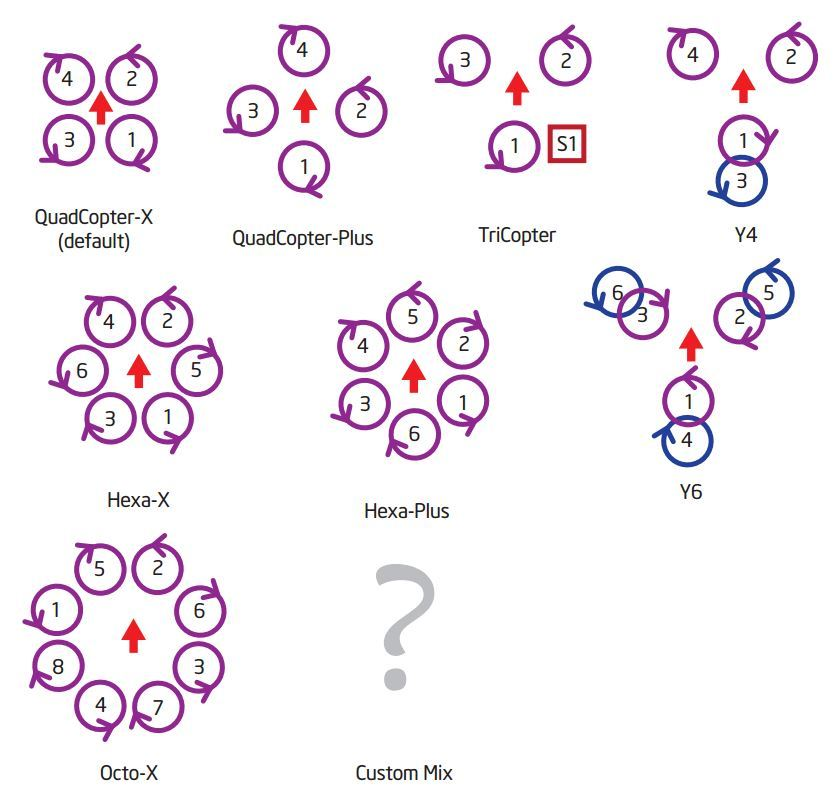
\includegraphics[scale=0.3]{fig/motor_layout.jpg}
	\label{fig:motor_layout}
	\caption{The motor layout for the mixers}
\end{figure}

\section{Saturation}

There are often agressive maneuvers which may cause multiple motor outputs to become saturated.  This is of particular concern in multirotors, and can be illustrated in the example of the command of maximum roll while at full throttle in a quadcopter.  Full throttle, with no other command, would normally cause all four motors to saturate at a maximum PWM command of 2000$\upmu$s.  Mixing in a maximum roll command would cause two of the motors to reduce to 1500$\upmu$s, while the other two would go to 2500$\upmu$s.  Because 2500$\upmu$s is beyond the maximum limit, the maximum roll command would actually be interpreted as a half-roll command as the difference between the motors on opposite sides of the MAV would be halved.  To increase controllability in these sorts of situations, we take the motor control value from the mixer, before it is shifted up 1000$\upmu$s to the standard PWM range, and find the scaling factor which would reduce the maximum motor command to 1000$\upmu$s.  We then apply this scaling factor to all other motors, and then shift them up to the standard PWM range of 1000$\upmu$s to 2000$\upmu$s.  This does not completely solve the problem, because the maximum roll command is still reduced somewhat, but it trades off maximum thrust for some additional controllability. In the case of a simultaneous maximum roll and maximum throttle, two of the motors will receive a command of 2000$\upmu$s, while the other two will receive a command of 1333$\upmu$s, as opposed to the 1500$\upmu$s without the saturation, and maintains controllability even at high levels of throttle.




\end{document}
